\documentclass[a4paper,10pt]{article}
\usepackage[utf8]{inputenc}
\usepackage{graphicx}
\graphicspath{{images/}}
\title{Final Project Proposal: Rap Machine}
\author{Nursultan Kabylkas, Ramesh Krishna Jayaraman, Ke Wang,\\ Yuan Yang, De Huo}

\begin{document}

\maketitle


We propose to implement two different neural net models, to perform different tasks of Image Captioning and Text/Poem Generation. As we are a group of five, the work will be divided evenly among us. Ke Wang, Yuan Yang, and De Huo will work on the CNN based model to perform image captioning. The output from that model will be used as input for the RNN based text/poem generation model, which will be implemented by Nursultan Kabylkas and Ramesh Jayaraman. The rest of this proposal will go into details about our proposed design, possible data set characteristics involved, and will provide a timeline for the work to be done. \\

\section{Proposed Design}

We are proposing to combine image captioning implemented with Convolution Neural Nets and poem generation implemented with Recurrent Neural Nets. 
The idea is to train CNN to caption images with sentences, and also train RNN with the song lyrics of different famous artists, such as: 2Pac, 50 cent, Snoop Dog, Coldplay, Tool, Iron Maiden etc. \\

Once the two Neural Net models are trained, we will use a test set of images to generate image caption, using the CNN model, and feed the generated text as an input of the RNN model, to generate the Poem/Lyrics. The purpose of this project is to evaluate the performance of RNN model, and compare generated lyrics among different artists, so as to compare their "style" of writing. 
Refer to Figure \ref{fig:architecture} to see the design.\\

\begin{figure}[h]
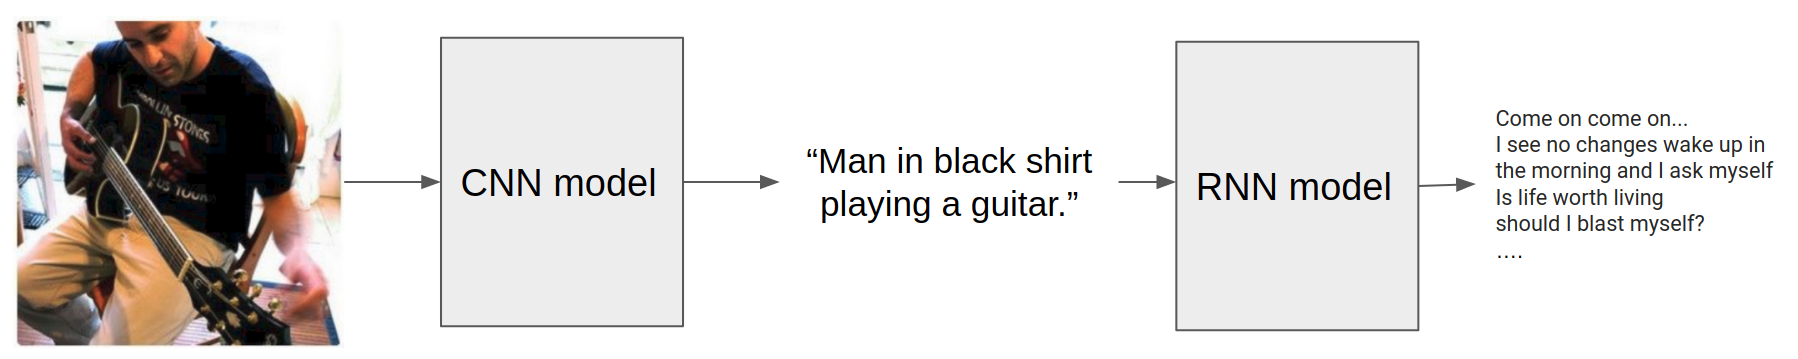
\includegraphics[scale=0.18]{figure1}
\caption{Architecture of the proposed implementation}
\label{fig:architecture}
\end{figure}

\section{Data Set Characteristics}

For the purposes of training/validating the CNN model for image captioning, we plan on using the Flickr8K, Flickr30K, and MSCOCO datasets. To train the RNN model for lyric/poem generation, we will use lyric datasets already available on Kaggle. We also might possibly use the same techniques used to gather the aforementioned datasets, to gather lyrics of artists if they are not in those datasets. 

\section{Timeline}

We would like to stick to the timeline shown in Figure \ref{fig:timeline}. 

\begin{figure}[h]
\centering
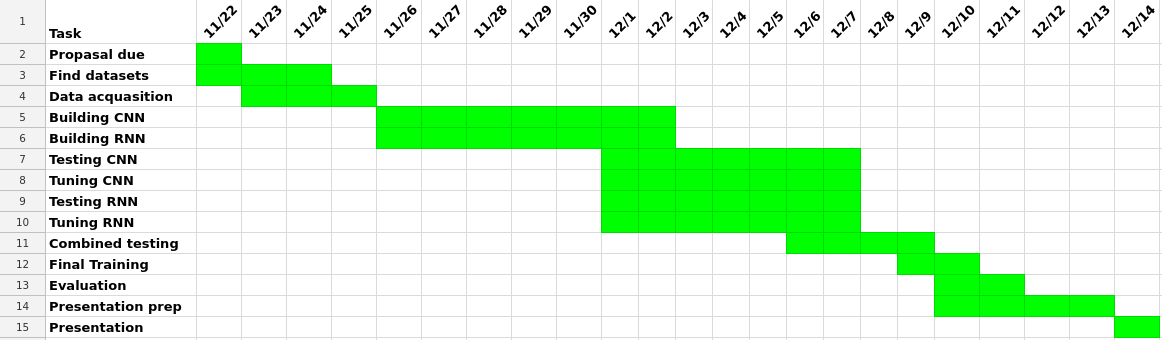
\includegraphics[scale=0.29]{timeline.png}
\caption{Timeline for proposed project.}
\label{fig:timeline}
\end{figure}




\end{document}
